\chapter{发电系统建模理论研究}
\label{cha:Modeling}

为了研究所提出的梯级系统的性能,使用EES(Engineering Equation Solver)和MATLAB(Matrix Laboratory)作为计算工具和开发工具创建了系统的模型。系统建模采用自底向上的设计方法。首先,在EES中建立机理模型用于来验证模型中各参数间的物理关系。其次,使用面向对象的方法在MATLAB中开发出部件模型,它充分利用了面向对象的封装性、继承性和多态性来保证部件之间的独立性和相关性。
依据不同流体,创建了三个回路(空气回路,水回路和油回路),并确定了一些关键部件的特定的状态参数。依据这些关键部件的热力学特性和动力学特性,为其创建了基于能量平衡的机理模型。

\section{发电系统部件建模}
\subsection{槽式集热器}
\label{sec:ptc}

槽式集热器由反射镜和接收器组成。反射镜(镜面)反射太阳直射辐射并将其会聚到位于抛物槽面焦线处的接收器上。接收器通常包含涂有高吸收率涂层的金属吸热管。在吸热管外部设有玻璃管以减少散热损失,吸热管和玻璃管之间通常被抽成真空以进一步减少热损。

在反射过程中存在着光学损失,它主要包含以下几项\cite{Price2002}:遮挡损失、跟踪损失、形状损失、反射率损失、镜面沾污损失。
%及其它未列入损失。
%\begin{itemize}
%  \item 遮挡损失
%  \item 跟踪损失
%  \item 形状损失
%  \item 反射率损失
%  \item 镜面沾污损失
%  \item 其它未列入损失
%\end{itemize}
此外还有一项,即太阳直射的阳光与集热器开口不垂直时,应该考虑入射角带来的损失($K(\theta)$,也称为余弦损失)。该损失是太阳入射角与集热器开口法线交角$\theta$的函数。
桑迪亚国家实验室的Dudley等\cite{Dudley1994}通过实验研究给出了槽式集热器的余弦损失计算公式:
\begin{equation}
  K(\theta) = \cos\theta+0.000884\theta-0.00005369\theta^2
\end{equation}

\autoref{fig:ParabolicTrough}给出了槽式集热器反射太阳光线的示意图,图中还标出了影响光学损失的一些参数。整个光学损失与下列五个参数有关:

\begin{enumerate}[label=(\arabic*)]
  \item 反射率,$\rho$:只有一部分入射辐射会被反射到接收器上。这一部分辐射量的多少由反射镜的种类决定。对于清洗干净的商业槽式反射镜,其反射率可以假定为0.9。
  \item 拦截因子,$\gamma$:由于反射镜的微观缺陷或抛物面槽式集热器的宏观形状误差,反射镜反射的太阳直射辐射中的一部分不能到达吸热管。这些缺陷或误差导致一些光线以错误的角度反射,因此它们不能被吸热管拦截吸收。这些损失通过称为拦截因子的光学参数来量化。对于正确组装的集热器而言,该参数通常为0.95。
  \item 透射率,$\tau$:到达接收器的玻璃管的太阳直射辐射只有一部分能够透射它。透射玻璃管的辐射与投射到其上的总的入射辐射之间的比称为透射率$\tau$,它通常取为0.93。
  \item 吸热管涂层的吸收率,$\alpha_{abs}$:该参数量化了吸热管吸收的能量与到达吸热管外壁的总辐射量的比例。对于有陶瓷涂层的金属吸热管,该参数通常为0.95,而对于涂有黑色镍或铬的吸热管,该参数值稍低。
  \item 沾污因子,$F_e$:反射镜上的污垢会降低反射率,因此需要考虑沾污带来的影响。沾污因子$F_e$的引入考虑了反射镜和玻璃管在清洗干净之后逐渐产生的沾污。
\end{enumerate}

\begin{figure}[!ht]
\centering
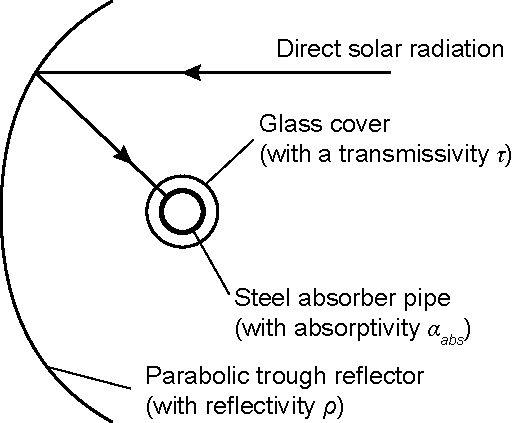
\includegraphics[width=0.3\textwidth]{fig/ParametersOfParabolicDish.pdf}
\caption{槽式集热器结构示意图}\label{fig:ParabolicTrough}
\end{figure}

穿透玻璃管到达吸热器的能量可以表示为
\begin{equation}
  P = I_r w_{tc} L_{tc} \rho \gamma \tau F_e K(\theta)
\end{equation}

为了简化吸热器的吸热过程,通常将其视为均匀的热流量$q''$
\begin{equation}
  q''= \frac{P}{\pi d_o L_{tc}} = \frac{I_r w_{tc} \rho \gamma \tau F_e K(\theta)}{\pi d_o}
\end{equation}

假设整体传热系数$U(T_{abs})$沿着整个集热器的长度方向是均匀的,可以将环境看作定温热源,这样就可以利用\autoref{cha:CTCHFHX}~中的传热计算公式计算吸热管对环境的散热。吸收管的传热分析示意图如\autoref{fig:Pipe}所示。
\begin{equation}
	\frac{T_{o}-T_{amb}-\dfrac{q''}{U(T_{abs})}}{T_{i}-T_{amb}-\dfrac{q''}{U(T_{abs})}}=\exp(-\frac{U(T_{abs})\pi d_o L_{tc}}{\dot{m}c_{p}})\label{eq:CTCHF}
\end{equation}

\begin{figure}[!ht]
\centering
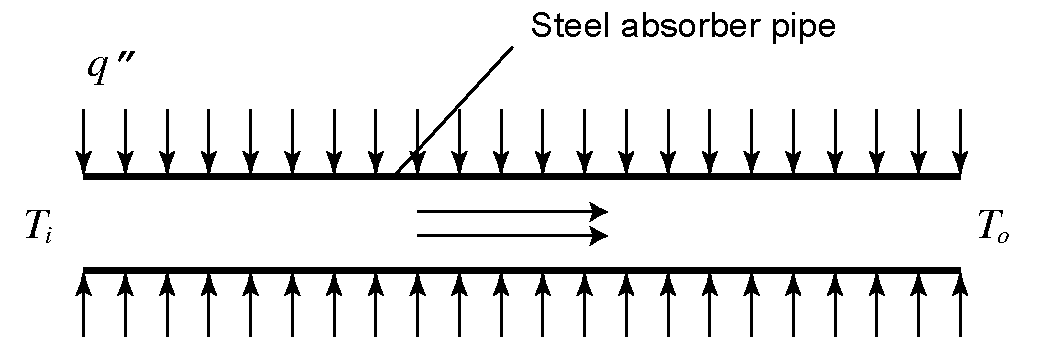
\includegraphics[width=0.6\textwidth]{fig/Pipe.pdf}
\caption{吸热管的传热分析示意图}\label{fig:Pipe}
\end{figure}

由于管道中的努塞尔数$Nu$非常大(大约为$1\times10^4$),吸热管和导热油之间的温差很小。所以平均流体温度$(T_{i}+T_{o})/2$可以用作吸热管温度$T_{abs}$的平均值,$U(T_{abs})$可以用Romero和Zarza给出的二阶多项式函数表示\cite{Romero2007}:
\begin{equation}
	U(T_{abs}) = 0.687257 + 0.001941(T_{abs} - T_{amb}) + 0.000026(T_{abs} - T_{amb})^2
\end{equation}

达到所需加热效果的槽式集热器的长度$L_{tc}$可以从\autoref{eq:CTCHF}中算得
\begin{equation}
	L_{tc} = \dfrac{\dot{m}c_p}{\pi d_o U(T_{abs})}\ln\left(\dfrac{T_i-T_{amb}-\dfrac{q''}{U(T_{abs})}}{T_o-T_{amb}-\dfrac{q''}{U(T_{abs})}}\right)
	\label{eq:get_L}
\end{equation}

垂直投射到槽式集热器开口的太阳辐射能为
\begin{equation}
  Q_{total} = I_r L_{tc} w_{tc}
\end{equation}

被传热流体吸收的能量为
\begin{equation}
  Q_{use} = \dot{m}c_p(T_o - T_i)
\end{equation}

槽式集热器的集热效率为
\begin{equation}
  \eta_{tc} = \dfrac{Q_{use}}{Q_{total}} = 
  \dfrac{I_r L_{tc} w_{tc}}{\dot{m}c_p(T_o - T_i)}
  \label{eq:eta_tc}
\end{equation}

基于以上简化假设和对槽式集热器的机理研究,本文建立了槽式集热器的模型。依据此模型可以方便地求解各类槽式集热器问题,并获得集热器的热效率。例如,已知传热流体进出口参数求解所需的集热器的长度,或者已知集热器长度和传热流体进口参数求解传热流体出口参数。

\subsection{碟式集热器}
\label{sec:pdc}

碟式集热器由反射镜和接收器组成。反射镜通过跟踪太阳来反射太阳光并将其会聚到位于反射镜焦点处的接收器。碟式集热器需要采用双轴跟踪系统来不间断地追踪太阳的轨迹。

碟式集热器的跟踪系统主要有两种型式\cite{Adkins1987}:
\begin{itemize}
  \item 由方位传感器进行的方位高度角跟踪,或由计算得到的太阳坐标通过控制系统进行控制。
  \item 极轴跟踪,集热器围绕与地轴平行的轴旋转跟踪太阳。
\end{itemize}

在传统的碟式斯特林机系统中,斯特林机放置在碟式集热器的焦点上。斯特林机设有接收器来吸收会聚的阳光。接收器由设有开孔的腔体和置于其中的吸热器组成。斯特林接收器的开孔位于反射器的焦点处,以减少辐射和对流损失。吸热器吸收太阳辐射能并将产生的热能传递给斯特林机的工作气体,为斯特林循环提供热量,使斯特林机的曲轴连续往复运动。直接连接到斯特林机曲轴的发电机将机械能转化为电能。

本文提出的梯级系统中,碟式集热器的焦点处放置有腔体式接收器。 一个金属螺旋管(称为吸热管)作为吸热器位于接收器中以吸收集中的太阳能。空气(或氮气)被用作传热流体流经吸热管以传输被吸热管吸收的能量,空气流出吸热器作为高温热源为其它部件提供热量。

碟式反射镜是碟式系统的重要元件。弯曲的反射表面可以利用单独的小型曲面拼接起来形成,或是通过由连续气室成形的拉伸膜形成。在所有的情况下,曲面都应镀铝或镀银以提高反射率。

本文选用SES(Stirling Energy System)公司生产的碟式反射镜作为梯级集热系统的碟式反射镜,其主要参数见于\autoref{tab:dc}。碟式接收器为自行设计研制的接收器,\autoref{fig:dishReceiver}是其结构示意图。

\begin{table}[htbp]
\setlength{\abovecaptionskip}{0pt}
	\caption{碟式集热器的主要参数}
	\centering
	\begin{tabular}{cccccc}
		\toprule
		参数		&	值	&	参数		&	值	&	参数		&	值\\
		\midrule
		$d_{cav}$	&	0.46$\,\mathrm{m}$	&	$\epsilon_{insu}$	&	0.6	&	$\theta_{dc}$	&	45$^\circ$\\
		$\delta_{insu}$	&	0.075$\,\mathrm{m}$	&	$\alpha_{cav}$	&	0.87	&	$\gamma$	&	0.97\\
		$l_{cav}$	&	0.23$\,\mathrm{m}$	&	$\delta_a$		&	0.005$\,\mathrm{m}$	&	$\eta_{shading}$	&	0.95\\
		$d_{ap}$	&	0.184$\,\mathrm{m}$	&	$d_{i,1}$	&	0.07$\,\mathrm{m}$	&	$\rho$	&	0.91\\
		$\lambda_{insu}$	&	0.06$\,\mathrm{W/(m\cdot K)}$	&	$A_{dc}$	&	87.7$\,\mathrm{m^2}$	&	\\		
		\bottomrule
	\end{tabular}
	\label{tab:dc}
\end{table}

\begin{figure}[!ht]
\centering
\includegraphics[width=0.4\textwidth]{fig/DishReceiver.pdf}
\caption{碟式接收器的结构示意图}\label{fig:dishReceiver}
\end{figure}

碟式接收器模型涉及的损失包括:接收器拦截损失,由于阴影造成的损失以及热损失。热损失占所有这些损失的最大部分,这部分损失由传导,对流和辐射三种形式组成。
\begin{figure}[ht!]
	\centering
	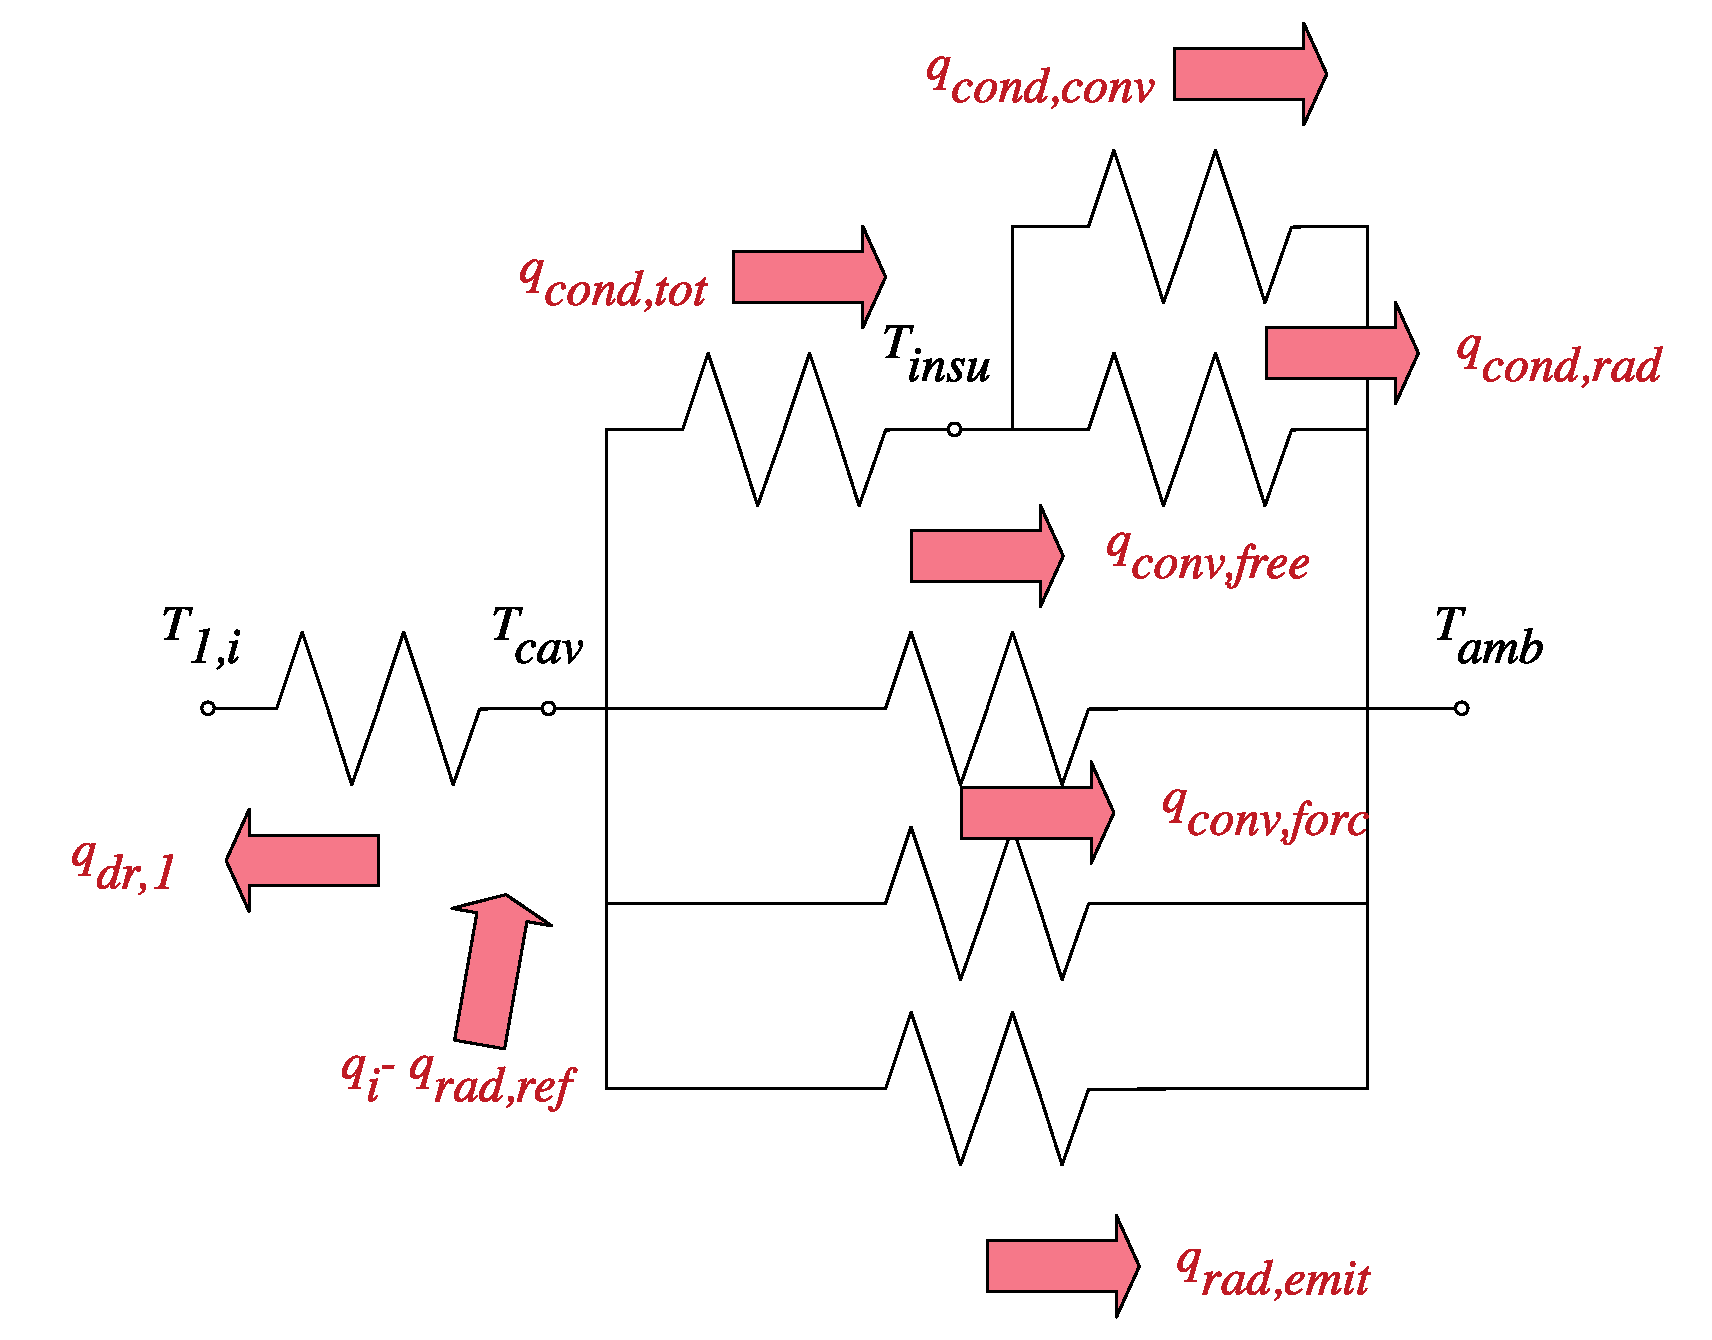
\includegraphics[width = 0.5\columnwidth]{fig/thermalLosses.pdf}
	\caption{碟式接收器的热网络模型}
	\label{fig:thermal-lose}
\end{figure}
为了详细分析碟式接收器的热损失,建立了如\autoref{fig:thermal-lose}所示的热网络模型。该网络模型考虑了以下损失:
\begin{itemize}
	\item 由接收器孔腔从接收器开口反射出去的辐射能损失,$q_{rad,ref}$。
	\item 由于和接收器的绝热层发生热传导产生的损失,$q_{cond,tot}$。
	\item 无风条件下接收器开口处发生的自然对流损失,$q_{conv,free}$。
	\item 有风条件下接收器开口处发生的强制对流损失,$q_{conv,forc}$。
	\item 由接收器孔腔发射出去的热辐射造成的辐射损失,$q_{rad,emit}$。
\end{itemize}

为了求解\autoref{fig:thermal-lose}中的热网络结构图,必须仔细分析图中各热流量的关系并求解方程。

\begin{enumerate}[label=(\arabic*)]
  \item \emph{入射到接收器的能量, $q_i$}
  
\setlength\parindent{2em}
为了简化模型,不考虑接收器对反射镜造成的遮挡,以及太阳跟踪系统的调节滞后造成的不利影响。
  \begin{equation}
      q_i = I_r A_{dc} \gamma \eta_{shading} \rho
      \label{eq:q_i}
  \end{equation}
其中,$\gamma$是拦截因子,$\eta_{shading}$是不同集热器之间遮挡造成的遮挡因子,$\rho$是反射镜的反射率。
  \item \emph{传热流体与吸热管之间的换热,$q_{dr,1}$}
  
  传热流体与吸热管之间的换热简化为经典的流体流过等壁温管道的换热模型。这样,$q_{dr,1}$可以由下式得到
  \begin{equation}
      q_{dr,1} = h_{dr,1}A_{dr,1}\Delta T_{ln,dr,1}
      \label{eq:q_dr_1}
  \end{equation}
  其中  
  \begin{equation}
      h_{dr,1} = Nu_{tube}\lambda_{dr,1} / d_{i,1}
\end{equation}
\begin{equation}
      Nu_{tube} = c_r Nu'_{tube}
\end{equation}
该式为修正后应用于螺旋管的努赛尔数计算公式,式中存在基于弯管曲率的螺旋因子$c_r$作为修正系数。$c_r$的表达式为\cite{Pablo2008}:
\begin{equation}
	c_{r}=1+3.5\frac{d_{i,1}}{d_{cav}-d_{i,1}-2\delta_{a}}
\end{equation}
$Nu'_{tube}$是直圆管的努塞尔数,它由下式计算\cite{Serth2007}:
\begin{equation}
	Nu'_{tube}= 0.027Re_{tube}^{0.8}Pr_{tube}^{1/3}(\mu_{tube}/\mu_{tube,w})^{0.14}
\end{equation}

传热流体与管壁之间的对数温差$\Delta{}T_{ln,dr,1}$可以写作
\begin{equation}
	\Delta{}T_{ln,dr,1}=\frac{(T_{cav}-T_{dc,i})-(T_{cav}-T_{dc,o})}{\ln\dfrac{T_{cav}-T_{dc,i}}{T_{cav}-T_{dc,o}}}
\end{equation}

  \item \emph{由接收器内壁从接收器开口反射出去的辐射能损失, $q_{rad,ref}$}
  \begin{equation}
    q_{rad,ref}=(1-\alpha_{eff})q_{i}
\end{equation}
    其中,$\alpha_{eff}$是接收器的等效吸收率,它由下式算得:
    \begin{equation}
    \alpha_{eff}=\frac{\alpha_{cav}}{\alpha_{cav}+(1-\alpha_{cav})\dfrac{A_{ap}}{A_{cav}}}
    \end{equation} 
$\alpha_{cav}$是接收器孔腔材料的吸收率,$A_{cav}$是孔腔的内表面总面积,$A_{ap}$是开口面积.
  \item \emph{由于和接收器的绝热层发生热传导产生的损失, $q_{cond,tot}$}
  
  \begin{equation}
q_{cond,tot}=2\pi\lambda_{insu}l_{cav}\dfrac{T_{cav}-T_{insu}}{\ln(1 + 2\delta_{insu}/d_{cav})}
    \end{equation}  
    其中,$T_{cav}$是孔腔的内壁温度,$T_{insu}$是绝热层的外壁温度。

  \item \emph{接收器绝热层的对流损失,$q_{cond,conv}$}  
  \begin{equation}
%\begin{split}
	q_{cond,conv}=h_{insu}A_{insu}(T_{insu}-T_{amb})
	=\dfrac{k_{insu}Nu_{insu}A_{insu}(T_{insu}-T_{amb})}{d_{cav}+2\delta_{insu}}
%\end{split}
\end{equation}
其中,$Nu_{insu}$可以由流体绕流圆柱体的公式得到\cite{Churchill1977}。

  \item \emph{接收器绝热层的辐射损失,$q_{cond,rad}$}  
  \begin{equation}
	q_{cond,rad}=\epsilon_{insu}A_{insu}\sigma(T_{insu}^4 - T_{amb}^4)
\end{equation}
  \item \emph{无风条件下接收器开口处发生的自然对流损失,$q_{conv,free}$}
    
  桑迪亚国家实验室进行了一系列实验,研究了不同工况下各种参数对碟式接收器开口处自然对流损失的影响,获取了大量的实验数据\cite{Ma1993}。这些数据同Stine和McDonald提出的自然对流公式获得的结果具有很高的一致性。本文假设的是强制对流和自然对流相互独立,所以强制对流和自然对流的综合对流损失如热网络结构图\autoref{fig:thermal-lose}所示。
  \begin{equation}
	q_{conv,free} = h_{free}A_{cav}(T_{cav}-T_{amb})
\end{equation}
其中,$h_{free}=k_{film}Nu_{free}/\overline{d_{cav}}$,$\overline{d_{cav}}$是孔腔的有效直径, 它由$\overline{d_{cav}}=d_{cav}-2d_i-4 \delta_a$算得。
$Nu_{free}由下式算得$\cite{Jilte2013b}:
\begin{equation}
	Nu_{free} = 0.088Gr^{1/3}(T_{cav}/T_{amb})^{0.18}\cos^{2.47}\theta (d_{ap}/\overline{d_{cav}})^S
\end{equation}
其中,
\begin{equation}
	S = -0.982d_{ap}/\overline{d_{cav}} + 1.12
\end{equation}
  
  \item \emph{有风条件下接收器开口处发生的强制对流损失,$q_{conv,forc}$}  
  \begin{equation}
	q_{conv,forc} = h_{forc}A_{cav}(T_{cav}-T_{amb})
\end{equation}

    Wu等\cite{Wu2010}针对碟式集热器的对流损失编写了全面的综述,并进行了系统性的总结。本文应用Leibfried和Ortjohann\cite{Leibfried1995}提出的改进型公式来计算接收器开口处的强制对流损失。该公式基于Koenig和Marvin\cite{Koenig1981}提出的公式、Stine和Diver\cite{Stine1994}提出的公式,并对一些影响因素进行了分析,具有更好的计算结果。

对于正面迎风,
\begin{equation}
	h_{forc}=0.1967v_{wind}^{1.849}
\end{equation}

对于侧面迎风,
\begin{equation}
	h_{forc}=f(\theta)v_{wind}^{1.401}
\end{equation}
\begin{equation}
	f(\theta)=0.1634 + 0.7498\sin\theta - 0.5026\sin(2\theta) + 0.3278\sin(3\theta)
\end{equation}
式中,$\theta$为风向与圆柱形接收器轴线间的夹角。

  \item \emph{由接收器孔腔发射出去的热辐射造成的辐射损失,$q_{rad,emit}$}
  
  孔腔被看作灰体,其辐射率和发射率相等,
\begin{equation}
    \epsilon_{cav}=\alpha_{eff}
\end{equation}
\begin{equation}
    q_{rad,emit}=\epsilon_{cav}A_{ap}\sigma(T_{cav}^{4}-T_{amb}^{4})
\end{equation}
\end{enumerate}

从热网络结构图(见\autoref{fig:thermal-lose})中可以得到
\begin{equation}
  q_{eff} = q_i - q_{rad,ref}
\end{equation}
\begin{equation}
  q_{eff} = q_{dr,1} + q_{cond,tot} + q_{conv,free} + q_{conv,forc}+q_{rad,emit}
\end{equation}
\begin{equation}
  q_{cond,tot} = q_{cond,conv}+q_{cond,rad}
\end{equation}

热网络结构图中的各温度节点可以通过上述方程解出。
$q_{dr,1}$可以通过\autoref{eq:q_dr_1}计算得出。于是,碟式接收器的热效率为
\begin{equation}
  \eta_{dr} = \frac{q_{dr,1}}{q_i}
\end{equation}

碟式集热器的热效率为
\begin{equation}
  \eta_{dc} = \frac{q_{dr,1}}{I_rA_{dc}}
\end{equation}

基于以上简化假设和对碟式集热器的机理研究,本文建立了碟式集热器的模型,模型可以方便地求解碟式接收器热网络图中的各种损失,并由此得到碟式集热器的集热效率。

\subsection{斯特林机}
\label{sec:StirlingEngineModel}
\subsubsection{斯特林循环}
理想斯特林循环由同冷热热源进行的两个等温换热过程及同回热器进行的两个定容换热过程组成。斯特林循环的$T$-$s$图如\autoref{fig:StirlingCycle}所示,图中4-1过程中回热器吸收的热量在2-3过程中被重新利用。但是实际上,由于回热过程不完善,这部分能量往往不能被完全利用,这部分能量只能将斯特林机的工作气体从2状态点加热到3'状态点,所以需要定义回热率$e$来表征回热器的完善程度\cite{Formosa2010,Juhasz2010}。$e=\dfrac{T_R-T_L}{T_H-T_L}$,其中$T_H$是热腔温度,$T_L$是冷腔温度,$T_R$是有效回热温度。

\begin{figure}[htbp]
\centering
	\includegraphics[width = 0.4\columnwidth]{fig/StirlingCycle}
	\caption{斯特林循环的$T$-$s$图}
	\label{fig:StirlingCycle}
\end{figure}

为了得到简化的分析模型,针对斯特林机做了以下简化假设:

\begin{itemize}
\item 斯特林机中的工质可以被看成理想气体。
\item 斯特林机不与环境间交换热量。
\item 冷热流体的平均换热系数为常数。
\item 回热器具有对称性,这样有效回热温度可以简化计算为$T_{R}=\dfrac{T_{H}-T_{L}}{\ln(T_{H}/T_{L})}$\cite{Formosa2010,Juhasz2010}。
\end{itemize}

为了考虑斯特林循环中由于存在死区容积带来的内部不可逆损失,将死区容积$V_D$划分成热头死区容积$V_{DH}$、回热器死区容积$V_{DR}$和冷头死区容积$V_{DC}$\cite{Duan2014},并采用容积因子$K$来描述不同温度下的各死区容积。$K$同各过程的温度及回热效率有关。

\begin{equation}
	K = \frac{V_{DH}}{T_H} + \frac{V_{DR}}{T_R} + \frac{V_{DC}}{T_L}
\end{equation}


对于定温压缩过程1-2,输出功
\begin{equation}
	W_{12} = \int^{V_E}_{V_E+V_C}{p_{12}dV}=-m_{se}RT_L\ln{\frac{V_E+V_C+KT_L}{V_E+KT_L}}
\end{equation}

对于定温膨胀过程3-4,输出功
\begin{equation}
	W_{34} = \int^{V_E+V_C}_{V_E}{p_{34}dV}=m_{se}RT_H\ln{\frac{V_E+V_C+KT_H}{V_E+KT_H}}
\end{equation}

定义$\gamma_H = \dfrac{V_E+V_C+KT_H}{V_E+KT_H}$,$\gamma_L = \dfrac{V_E+V_C+KT_L}{V_E+KT_L}$。在一个循环过程中,理论输出功
\begin{equation}
	W_{th} = W_{12} + W_{34} = m_{se}R(T_H\ln\gamma_H - T_L\ln\gamma_L)
\end{equation}

对于定容加热过程3'-3,吸收的热量
\begin{equation}
	\begin{split}
		Q_{3^{'}3} = nc_v(T_H-T_R)
%		\\=n(1-e)c_v(T_H-T_L)
		=\frac{1-e}{k-1}m_{se}R(T_H-T_L)
	\end{split}
\end{equation}

对于定温膨胀过程3-4,吸收的热量
\begin{equation}
	Q_{34} = W_{34} = m_{se}RT_H\ln\gamma_H
\end{equation}

在一个循环过程中,理论吸收热为
\begin{equation}
	Q_{th} = Q_{3^{'}3} + Q_{34} = \frac{1-e}{k-1}m_{se}R(T_H-T_L) + m_{se}RT_H\ln\gamma_H
\end{equation}

\subsubsection{不可逆因素及损失}

本文主要考虑以下不可逆因素及损失:
\begin{enumerate}[label=(\arabic*)]
\item \emph{非理想传热影响}

\setlength\parindent{2em}
由于加热器和冷却器的传热过程并非理想传热,它们的流体同换热器壁面间存在温差。加热器中的热流体温度$T_{H}$要高于加热器的壁面温度$T_{hw}$,冷却器中的冷却流体温度$T_L$要低于冷却器的壁面温度$T_{cw}$。根据传热学,$T_{H}$和$T_{L}$可以通过下式修正:

\begin{equation}
	T_H = T_{hw} - \frac{Qs_{se}}{h_hA_{hw}}
	\label{eq:T_H}
\end{equation}
\begin{equation}
	T_L = T_{cw} + \frac{(Q-W)s_{se}}{h_cA_{cw}}
	\label{eq:T_L}
\end{equation}

其中的传热系数可以通过下式获得\cite{Babaelahi2015}:
\begin{equation}
	h_{h,c} = \frac{\mu c_pf_{Re}}{2D_{h,c}Pr_{h,c}}
\end{equation}
式中,$f_{Re}$是与雷诺数有关的摩擦因子:
\begin{equation}
	f_{Re} = 0.0791Re_{h,c}^{0.75}
\end{equation}
$Re_{h,c}$,$Pr_{h,c}$和$D_{h,c}$分别是加热器/冷却器的雷诺数,普朗特数和水利直径。

\item \emph{压力损失带来的影响}

压力损失使斯特林机的输出功率下降。压力损失可以表示为\cite{Urieli1984}:
\begin{equation}
	\Delta p = -\frac{2f_{Re}\mu u V}{d^2A}
\end{equation}
其中,$u$是工作气体的流速,$V$是流通体积,$A$是流动截面积。

由压力损失带来的斯特林机的净输出损失可以由下式计算得到:
\begin{equation}
	W_{pd} = \oint\underset{i = E,C}{\sum}(\Delta p_{i}\frac{dV_i}{d\theta})d\theta
\end{equation}

\item \emph{由于活塞运动及机械摩擦带来的损失}

由于活塞的运动,压缩过程和膨胀过程中活塞表面的压力与气体压力不同。可以证明,压缩过程中活塞表面的压力要高于气体压力,膨胀过程中活塞表面的压力要低于气体压力。这意味着输出功要少于理论值。此外,机械摩擦的存在也会减少输出功率。由于活塞运动及机械摩擦带来的损失可以由下式得到\cite{Babaelahi2015}:
\begin{equation}
	W_{fs} = \oint p(\pm\frac{au_p}{c}\pm\frac{\Delta p_f}{p})dV
\end{equation}
其中,加号($+$)用于压缩过程,减号($-$)用于膨胀过程。$p$是压缩腔和膨胀腔的平均压力,$u_p$是活塞的速度,$c$是气体分子的平均速度,$\Delta p_f$是由于机械摩擦导致的压力损失。$\Delta p_f$,$a$和$c$可以由下列各式得到\cite{Heywood1988}:

\begin{equation}
	\Delta p_f = 0.97+0.009s_{se}
\end{equation}
\begin{equation}
	a = \sqrt{3k}
\end{equation}
\begin{equation}
	c = \sqrt{3RT}
\end{equation}

\item \emph{由于内部导热引起的能量损失}

由于加热器和冷却器存在温差,会有热量以导热的形式透过回热器壁进行传输\cite{Strauss2010}。在一个循环周期中,由于内部导热引起的损失可以由下式得到:
\begin{equation}
	Q_{id} = \frac{k_rA_r}{L_rs_{se}}(T_{hw} - T_{cw})
\end{equation}
其中,$k_r$、$L_r$和$A_r$分别表示回热器的导热率、长度和导热面积。

\item \emph{穿梭导热产生的能量损失}

由于置换器在膨胀腔和压缩腔中往来穿梭,它会在热端区间吸热,在冷端区间放热。这部分损失可以由下式估算\cite{Timoumi2008}:
\begin{equation}
	Q_{sc} = 0.4\frac{Z^2k_pD_p}{JL_ds_{se}}(T_{H} - T_{L})
\end{equation}
其中,$Z$、$k_p$、$D_p$、$J$和$L_d$分别表示置换器的往复长度、活塞导热率、置换器的直径、置换器和圆柱体内壁之间的缝隙大小以及置换器的长度。

\end{enumerate}

于是,斯特林机在一个循环过程中的总吸热量可以表述为
\begin{equation}
	Q = Q_{th} + Q_{id} + Q_{sc}
	\label{eq:heat}
\end{equation}

总的输出功可以表述为
\begin{equation}
	W = W_{th} - W_{pd} - W_{fs}
	\label{eq:work}
\end{equation}

斯特林机的输出功率为
\begin{equation}
	P = Ws_{se}
	\label{eq:P}
\end{equation}

斯特林机的效率为
\begin{equation}
	\eta = W/Q
	\label{eq:eta}
\end{equation}

\subsubsection{斯特林机与冷热流体间的传热}

对于斯特林机的传热过程,加热器、冷却器和回热器的壁面温度被假定为均匀且恒定。于是可以利用\autoref{cha:CTHX}~中的流体与定温热源的传热计算公式,有
\begin{equation}
	\frac{T_o-T_w}{T_i-T_w}=\exp(-\frac{UA}{\dot{m}c_p})
\end{equation}

对于斯特林机,可以分别用$T_{hw}$和$T_{cw}$来替代$T_w$,用$T_{i,h}$、$T_{o,h}$及$T_{i,c}$、$T_{o,c}$来替代$T_{i}$与$T_{o}$。
\begin{equation}
	\frac{T_{o,h}-T_{hw}}{T_{i,h}-T_{hw}}=\exp(-\frac{U_hA_h}{\dot{m}_hc_{p,h}})
	\label{eq:T_h}
\end{equation}
\begin{equation}
	\frac{T_{o,c}-T_{cw}}{T_{i,c}-T_{cw}}=\exp(-\frac{U_cA_c}{\dot{m}_cc_{p,c}})
	\label{eq:T_c}
\end{equation}

斯特林机的热流体的出口温度
\begin{equation}
	T_{o,h}=(T_{i,h}-T_{hw})\exp(-\frac{U_hA_h}{\dot{m}_hc_{p,h}}) + T_{hw}
	\label{eq:T_o_h}
\end{equation}

斯特林机的热流体的出口温度
\begin{equation}
	T_{o,c}=(T_{i,c}-T_{cw})\exp(-\frac{U_cA_c}{\dot{m}_cc_{p,c}}) + T_{cw}
	\label{eq:T_o_c}
\end{equation}

在一个循环周期中,热流体传递给斯特林机的热量为
\begin{equation}
	Q = \dot{m}_hc_{p,h}(T_{i,h}-T_{o,h})/s_{se}
	\label{eq:q_h}
\end{equation}

在一个循环周期中,斯特林机传递给冷流体的热量为
\begin{equation}
	 Q - W = \dot{m}_cc_{p,c}(T_{o,c}-T_{i,c})/s_{se}	\label{eq:q_c}
\end{equation}

基于以上简化假设和对斯特林机循环及其各种不可逆因素损失的分析,本文建立了斯特林机的模型。依据此模型可以求解给定斯特林机及其冷热流体条件下,斯特林机的输出功率和效率。并可以得到冷热流体流出斯特林机后的状态信息。

\subsubsection{模型验证}
\label{sec:modelValidation}

通过选用GPU-3型斯特林机作为实例,对所建立的模型进行评估。GPU-3型斯特林机的设计参数见\autoref{tab:GPU3parameters}\cite{Babaelahi2015,Martini1983}。将建立的模型计算得到的斯特林机效率和功率同经典模型及实验结果进行比较,结果如\autoref{tab:EfficiencyComparison}和\autoref{tab:PowerComparison}所示。

\begin{table*}[t!]\footnotesize
\setlength{\abovecaptionskip}{0pt}
	\caption{GPU-3型斯特林机的设计参数}
	\centering
	\begin{tabular}{ll}
		\toprule
		参数				&	值\\
		\midrule
		斯特林机类型					&	$\beta$型\\
		工作气体			&	氦气\\
		工作气体的质量	&	1.136\,g\\
		\emph{加热器}			&\\
		管道数量		&	40\\
		管道外径	&	4.83$\times$10$^{-3}\,\mathrm{m}$\\
		管道内径	&	3.02$\times$10$^{-3}\,\mathrm{m}$\\
		管道长度(圆柱体部分)		&	0.1164\,m\\
		管道长度 (回热器部分)		&	0.1289\,m\\
		\emph{冷却器}			&\\
		管道数量		&	312\\
		管道外径	&	1.59$\times$10$^{-3}\,\mathrm{m}$\\
		管道内径	&	1.09$\times$10$^{-3}\,\mathrm{m}$\\
		平均管道长度		&	4.61$\times$10$^{-2}\,\mathrm{m}$\\
		\emph{回热器}		&\\
		回热器数量	&	8\\
		回热器内径	&	2.26$\times$10$^{-2}\,\mathrm{m}$\\
		回热器长度		&	2.26$\times$10$^{-2}\,\mathrm{m}$\\
		%回热器管径	&	4$\times$10$^{-5}\,\mathrm{m}$\\
		材料				&	不锈钢\\
		\emph{容积}			&\\
		波及容积(膨胀/压缩)	&	120.82/114.13$\,\mathrm{cm}^3$\\
		余隙容积(膨胀/压缩)	&	30.52/28.68$\,\mathrm{cm}^3$\\
		死区容积(加热器/冷却器/回热器)	&	70.28/13.18/50.55$\,\mathrm{cm}^3$\\
		\bottomrule
	\end{tabular}
	\label{tab:GPU3parameters}
\end{table*}

\begin{sidewaystable}[htbp]\footnotesize
\setlength{\abovecaptionskip}{0pt}
  \renewcommand\arraystretch{0.75}
	\caption{模型及实验的热效率($T_{hw}=$922$\,\mathrm{K}$,$T_{cw}=$288$\,\mathrm{K}$)}
	\centering
	\begin{tabular}{cccccccccccc}
		\toprule
		\multirow{5}{0.5in}{\tabincell{c}{转速\\(Hz)}}	&
    \multirow{5}{0.5in}{平均\\ 有效\\ 压力\\ (MPa)}	&	\multicolumn{3}{c}{\multirow{2}{1.4in}{简单分析模型\\(变普朗特数\cite{Urieli1984})}}	&	\multicolumn{3}{c}{\multirow{2}{1.4in}{绝热分析模型 (simple II\cite{Strauss2010})}}	&	\multicolumn{3}{c}{\multirow{2}{1.4in}{本文提出的模型}}	&	\multirow{2}{*}{\tabincell{c}{实验\\数据\cite{Babaelahi2015}}}\\
    \\
    \\
		\cline{3-12}
		&&\multirow{3}{*}{\tabincell{c}{数值\\(\%)}}&	\multirow{3}{*}{\tabincell{c}{误差\\(\%)}}&\multirow{3}{*}{\tabincell{c}{平均\\误差\\(\%)}}&\multirow{3}{*}{\tabincell{c}{数值\\(\%)}}&	\multirow{3}{*}{\tabincell{c}{误差\\(\%)}}&\multirow{3}{*}{\tabincell{c}{平均\\误差\\(\%)}}&\multirow{3}{*}{\tabincell{c}{数值\\(\%)}}&	\multirow{3}{*}{\tabincell{c}{误差\\(\%)}}&\multirow{3}{*}{\tabincell{c}{平均\\误差\\(\%)}}&\multirow{3}{*}{\tabincell{c}{实际\\数值\\(\%)}}\\
		\\
		\\
		\midrule
		16.67	&\multirow{6}{*}{2.76}	&38.72	&18.22	&\multirow{6}{*}{17.90}	&32.48	&11.98	&\multirow{6}{*}{12.85}	&28.16	&7.66	&\multirow{6}{*}{12.10}	&20.50\\
		25.00	&&36.16	&15.46	&&31.21	&10.51	&&27.75	&7.05	&&20.70\\
		33.33	&&33.79	&15.79	&&29.45	&11.45	&&27.43	&9.43	&&18.00\\
		41.67	&&31.48	&16.28	&&27.45	&12.25	&&27.17	&11.97	&&15.20\\
		50.00	&&29.12	&17.32	&&25.21	&13.41	&&26.94	&15.14	&&11.80\\
		58.33	&&29.74	&24.34	&&22.89	&17.49	&&26.74	&21.34	&&5.40\\
		\midrule
		25.00	&\multirow{5}{*}{4.14}	&35.65	&10.85	&\multirow{5}{*}{11.46}	&32.29	&7.49	&\multirow{5}{*}{8.28}	&27.29	&2.49	&\multirow{5}{*}{6.65}	&24.80\\
		33.33	&&33.52	&9.62	&&30.40	&6.50	&&26.94	&3.04	&&23.90\\
		41.67	&&31.48	&10.18	&&28.39	&7.09	&&26.65	&5.35	&&21.30\\
		50.00	&&29.45	&11.25	&&26.33	&8.13	&&26.39	&8.19	&&18.20\\
		58.33	&&27.40	&15.40	&&24.21	&12.21	&&26.17	&14.17	&&12.00\\
		\midrule
		41.67	&\multirow{3}{*}{5.52}	&31.20	&8.70	&\multirow{3}{*}{10.82}	&28.59	&6.09	&\multirow{3}{*}{8.11}	&26.24	&3.74	&\multirow{3}{*}{7.48}	&22.50\\
		50.00	&&29.33	&10.53	&&26.62	&7.82	&&25.97	&7.17	&&18.80\\
		58.33	&&27.44	&13.24	&&24.62	&10.42	&&25.73	&11.53	&&14.20\\
		\midrule
		50.00	&\multirow{2}{*}{6.90}	&29.07	&10.37	&\multirow{2}{*}{11.73}	&26.61	&7.91	&\multirow{2}{*}{9.19}	&25.62	&6.92	&\multirow{2}{*}{9.05}		&18.70\\
		58.33	&&27.29	&13.09	&&24.67	&10.47	&&25.37	&11.17	&&14.20\\
		\bottomrule
	\end{tabular}
	\label{tab:EfficiencyComparison}
\end{sidewaystable}

\begin{sidewaystable}[htbp]\footnotesize
\setlength{\abovecaptionskip}{0pt}\
  \renewcommand\arraystretch{0.75}
	\caption{模型及实验的输出功率($T_{hw}=$922$\,\mathrm{K}$,$T_{cw}=$288$\,\mathrm{K}$)}
	\centering
	\begin{tabular}{cccccccccccc}
		\toprule
		\multirow{5}{0.5in}{\tabincell{c}{转速\\(Hz)}}	&
    \multirow{5}{0.5in}{平均\\ 有效\\ 压力\\ (MPa)}	&	\multicolumn{3}{c}{\multirow{2}{1.4in}{简单分析模型\\(变普朗特数\cite{Urieli1984})}}	&	\multicolumn{3}{c}{\multirow{2}{1.4in}{绝热分析模型 (simple II\cite{Strauss2010})}}	&	\multicolumn{3}{c}{\multirow{2}{1.4in}{本文提出的模型}}	&	\multirow{2}{*}{\tabincell{c}{实验\\数据\cite{Babaelahi2015}}}\\
    \\
    \\
		\cline{3-12}
		&&\multirow{3}{*}{\tabincell{c}{数值\\(kW)}}&	\multirow{3}{*}{\tabincell{c}{误差\\(\%)}}&\multirow{3}{*}{\tabincell{c}{平均\\误差\\(\%)}}&\multirow{3}{*}{\tabincell{c}{数值\\(kW)}}&	\multirow{3}{*}{\tabincell{c}{误差\\(\%)}}&\multirow{3}{*}{\tabincell{c}{平均\\误差\\(\%)}}&\multirow{3}{*}{\tabincell{c}{数值\\(kW)}}&	\multirow{3}{*}{\tabincell{c}{误差\\(\%)}}&\multirow{3}{*}{\tabincell{c}{平均\\误差\\(\%)}}&\multirow{3}{*}{\tabincell{c}{实际\\数值\\(kW)}}\\
		\\
		\\
		\midrule
		16.67	&\multirow{6}{*}{2.76}	&1.796	&119.02	&\multirow{6}{*}{272.03}	&1.772	&116.10	&\multirow{6}{*}{254.71}	&0.861	&4.98	&\multirow{6}{*}{104.84}	&0.82\\
		25.00	&&2.555	&128.13	&&2.500	&123.21	&&1.253	&11.88	&&1.12\\
		33.33	&&3.215	&165.70	&&3.117	&157.60	&&1.632	&34.88	&&1.21\\
		41.67	&&3.769	&211.49	&&3.615	&198.76	&&2.001	&65.37	&&1.21\\
		50.00	&&4.195	&303.37	&&3.973	&282.08	&&2.362	&127.12	&&1.04\\
		58.33	&&4.505	&704.46	&&4.203	&650.54	&&2.715	&384.82	&&0.56\\
		\midrule
		25.00	&\multirow{5}{*}{4.14}	&3.844	&114.75	&\multirow{5}{*}{259.70}	&3.761	&110.11	&\multirow{5}{*}{158.41}	&1.818	&1.56	&\multirow{5}{*}{39.83}	&1.79\\
		33.33	&&4.856	&120.73	&&4.708	&114.00	&&2.362	&7.36	&&2.20\\
		41.67	&&5.734	&136.94	&&5.501	&127.31	&&2.890	&19.42	&&2.42\\
		50.00	&&6.462	&174.98	&&6.126	&160.68	&&3.405	&44.89	&&2.35\\
		58.33	&&7.030	&306.36	&&6.573	&279.94	&&3.908	&125.90	&&1.73\\
		\midrule
		41.67	&\multirow{3}{*}{5.52}	&7.645	&133.08	&\multirow{3}{*}{180.02}	&7.334	&123.60	&\multirow{3}{*}{164.91}	&3.742	&14.09	&\multirow{3}{*}{43.68}	&3.28\\
		50.00	&&8.655	&163.87	&&8.206	&150.18	&&4.401	&34.18	&&3.28\\
		58.33	&&9.470	&243.12	&&8.858	&220.94	&&5.045	&82.79	&&2.76\\
		\midrule
		50.00	&\multirow{2}{*}{6.90}	&10.788	&174.50	&\multirow{2}{*}{287.04}	&10.223	&160.13	&\multirow{2}{*}{263.63}	&5.362	&36.44	&\multirow{2}{*}{97.75}		&3.93\\
		58.33	&&11.840	&399.58	&&11.071	&367.13	&&6.140	&159.07	&&2.37\\
		\bottomrule
	\end{tabular}
	\label{tab:PowerComparison}
\end{sidewaystable}

从表中可以发现,与之前的斯特林机热力模型相比,本文建立的模型同实验在不同转速和不同平均有效压力的条件下得到的结果更加接近。需要指出的是,上述所有模型中,输入热量$Q$和输出功率$W$都由工作气体同壁面的换热得到。在本文建立的模型中,$Q$和$W$由\autoref{eq:heat}和\autoref{eq:work}得到。因此,$Q$,$W$和$\eta$都可以由热力模型和输入参数得到。这些输入参数包括加热器参数、冷却器参数、回热器参数、平均有效压力、工作气体的类型以及斯特林机的几何尺寸。

\autoref{tab:EfficiencyComparison}和\autoref{tab:PowerComparison}表明,当斯特林机的平均有效压力位于2.76$\,\mathrm{MPa}$到6.90$\,\mathrm{MPa}$之间时,本文建立的模型具有最佳性能预测准确性。当斯特林机的转速从16.67$\,\mathrm{Hz}$增加到58.33$\,\mathrm{Hz}$时,本文建立的模型的性能预测的误差也随之增大。所以本文所建立的模型在平均有效压力在2.76$\,\mathrm{MPa}$和6.90$\,\mathrm{MPa}$之间,转速较低时具有最佳性能预测准确性。

然而,同实验结果相比,本文提出的模型仍然存在一些误差。未来的研究工作可能会考虑斯特林机的其它不可逆损失,如斯特林机向环境的散热,气弹滞后效应等等,从而建立更加精确的斯特林机模型。值得指出的是,其它文献也有提到更加精确的斯特林机模型。例如,多变过程模拟模型具有比本文提出的模型更高的性能预测精度\cite{Hosseinzade2015, Babaelahi2015}。然而,该模型需要假定斯特林循环中各过程的多变指数,该多变指数又与具体的斯特林机及具体的过程相关,而且多变过程模拟模型需要更多的计算量。

\section{朗肯循环发电子系统建模}
%The power generating system includes the turbine (steam turbine or ORC 
依据工作流体的不同,存在两种不同的朗肯循环发电子系统——水工质朗肯循环子系统和有机工质朗肯循环子系统。

\subsection{水工质朗肯循环}
  
  水工质朗肯循环需要设置除氧器以去除给水中的氧气和其它不凝结气体。给水中溶解的氧气将会给蒸汽发生系统造成严重的腐蚀损伤,并使金属管道形成氧化物(生锈)。溶解在给水中的二氧化碳将会形成碳酸,并进一步对管道造成腐蚀。不凝结气体的聚集将会增加热阻,这对各种换热器很不利。本系统中的除氧器采用汽轮机抽汽作为热源。
  
\begin{figure}[!ht]
\centering
	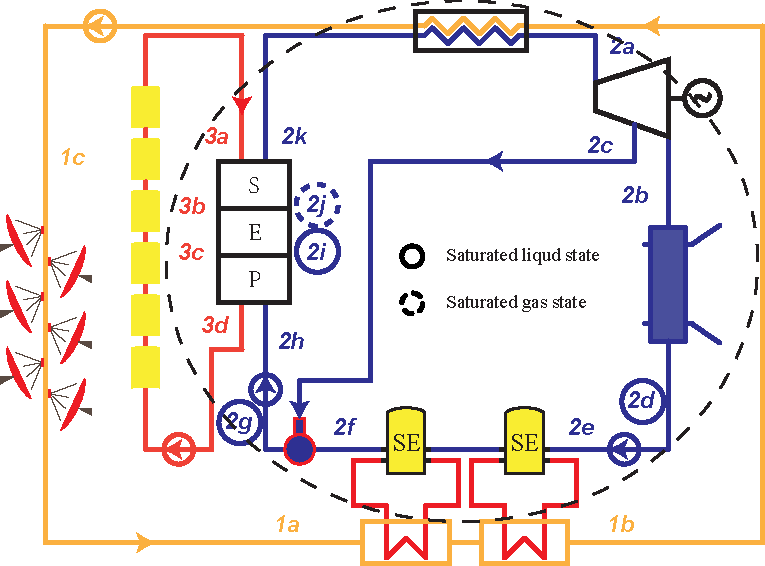
\includegraphics[width = 0.8\columnwidth]{fig/SRCinCS}
	\caption{用于分析水工质朗肯循环的梯级系统结构示意图}
	\label{fig:SRCinCS}
\end{figure}
  
  以\autoref{fig:SRCinCS}为例,详细介绍水工质朗肯循环的建模理论研究。\autoref{fig:SRCinCS}中,各种流体的不同状态点用数字加字母标出。其中,数字表示流体类型:1代表空气,2代表水,3代表导热油;字母代表不同位置的状态点。有的状态点还加有圆圈,表示其为饱和状态:实线圆圈表示为饱和液态,$x = 0$;虚线圆圈表示为饱和气态,$x = 1$。

梯级系统的水循环的温熵图如\autoref{fig:Ts_Water1}所示。过程曲线$2a$-$2c$-$2b$表示汽轮机内蒸汽做功的过程,其焓熵曲线图如\autoref{fig:SteamTurbine_hs}所示。状态点$2b$和$i,2b$的压力相等,状态点$2c$和$i,2c$的压力相等。为了简化汽轮机内效率的计算,假定汽轮机在不同负荷、不同级中的相对内效率不变,即
\begin{equation}
      \eta_{i,tb} =(h_{2a}-h_{2b})/(h_{2a}-h_{i,2b}) = (h_{2a}-h_{2c})/(h_{2a}-h_{i,2c})
\end{equation}
其中,$h_{i,2b}$由$s_{2a}$和$p_c$得到,$h_{i,2c}$由$s_{2a}$和$p_e$得到。

  汽轮机的输出功率
  \begin{equation}
  P_{tb}=\left(1-y\right)\dot{m}_{2}\left(h_{2a}-h_{2b}\right)+y\dot{m}_{2}\left(h_{2a}-h_{2c}\right)
  \end{equation}
 
  \noindent \begin{figure}[htbp]
\centering
	\begin{subfigure}[b]{0.6\columnwidth}
	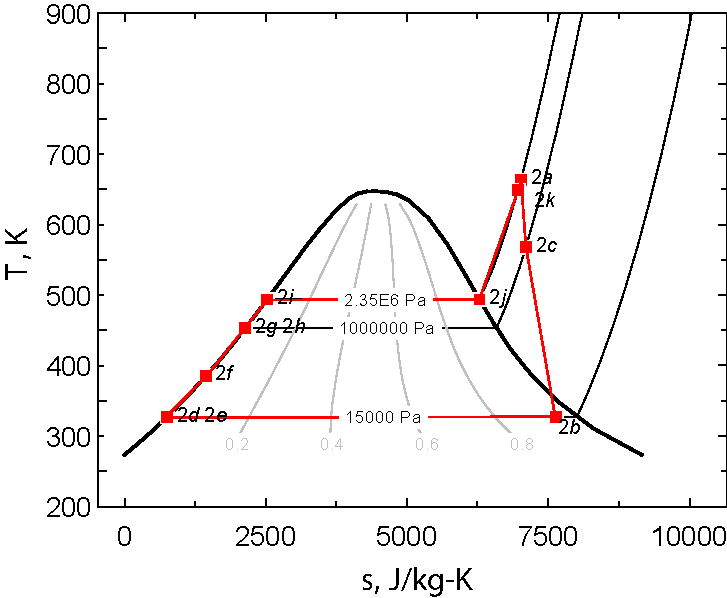
\includegraphics[width = \columnwidth]{fig/T-s_Water.pdf}
	\caption{}\label{fig:Ts_Water1}
	\end{subfigure}
	~
\begin{subfigure}[b]{0.28\columnwidth}
	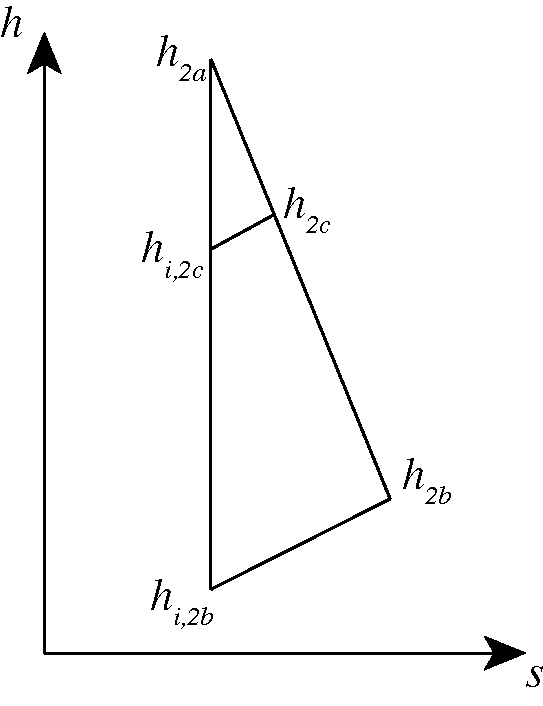
\includegraphics[width = \columnwidth]{fig/SteamTurbine_hs.pdf}
	\caption{}\label{fig:SteamTurbine_hs}
	\end{subfigure}
	\caption{水循环的$T$-$s$图及过程$2a$-$2c$-$2b$的$h$-$s$图}\label{fig:SteamTurbine_hs_p}
\end{figure}

  过程$2b$-$2d$表示凝汽器中的换热工况。凝汽器的出口水是饱和液态水,其出口温度$T_{2d}$和出口焓值$h_{2d}$由汽轮机的排汽压力$p_c$确定。
  凝汽器释放的热量
  \begin{equation}
      Q_{cd} = (1-y)\dot{m}_2 (h_{2b} - h_{2d})
\end{equation}

  除氧器的各进口压力和出口压力相等,状态点$2c$、$2f$和$2g$具有相同的压力(等于$p_e$)。除氧器的出口水是饱和液态水,其焓值可以由$p_e$确定。
  由能量平衡方程
  \begin{equation}
  y h_{2c} + (1-y) h_{2f} = h_{2g}
\end{equation}
 
  泵消耗的总功率
\begin{equation}
	P_{pu}=\left(1-y\right)\dot{m}_{2}\left(h_{2e}-h_{2d}\right)+\dot{m}_{2}\left(h_{2h}-h_{2g}\right)
\end{equation}   
其中,$h_{2e}$可以通过方程$\eta_{pu} = (h_{i,2e}-h_{2d})/(h_{2e}-h_{2d})$获得,$h_{2h}$可以通过方程$\eta_{pu} = (h_{i,2h}-h_{2g})/(h_{2h}-h_{2g})$获得。$h_{i,2e}$由$s_{2d}$和$p_e$决定,$h_{i,2h}$由$s_{2g}$和$p_s$决定。

由于除氧器的出口水是饱和液态水,其出口温度$T_{2g}$和出口焓值$h_{2g}$由除氧器的压力$p_{2g}$决定。
\begin{equation}
  p_{2g} = p_{2c}
\end{equation}
    
水循环吸收的总热量为
\begin{equation}
	Q_2=\left(1-y\right)\dot{m}_{2}\left(h_{2f}-h_{2e}\right)+\dot{m}_{2}\left(h_{2a}-h_{2h}\right)
\end{equation}

朗肯循环的效率可以表示为
\begin{equation}
	\eta_{rk}=(P_{tb}-P_{pu}/\eta_{ge})/Q_{2}
\end{equation}

\subsection{有机工质朗肯循环}
  
不同有机工质的饱和$T$-$s$图具有不同形状的饱和曲线。有机工质可以根据$T$-$s$图中饱和蒸气曲线斜率$dT/ds$的不同分为三种类型:$dT / ds > 0$表示该流体为干工质(高压饱和蒸气定熵膨胀时不会进入湿气区),大多数有机工质为干工质;$dT / ds < 0$表示该流体为湿工质(高压饱和蒸气定熵膨胀时会产生液滴),少数有机工质为湿工质;$dT/ds \rightarrow \pm\infty$表示该流体为等熵流体,例如R134a。对于干工质,由于在汽轮机中不会出现液滴,有机工质无需过热。此外,对于应用于低温废热回收的有机工质朗肯循环,也无需进行过热。由于本文讨论的太阳能光热发电技术所获得的集热温度一般高于有机工质的饱和温度,所以本文选用的有机工质朗肯循环仍然采用过热,以提高朗肯循环的效率。

水工质朗肯循环和典型有机工质朗肯循环的$T$-$s$图分别如\autoref{fig:Ts_Water}和\autoref{fig:Ts_organic}所示。在典型有机工质循环(其系统结构图如\autoref{fig:ORCsystem2})中,循环效率可以通过使用回热器来得到提升。这是因为汽轮机出口工质是过热气体,其温度比对应压力下的凝汽温度高。利用这部分高出的温度可以给加压的凝结液提供热量。通常会在有机工质汽轮机的出口和蒸发器的进口之间安装一个逆流布置的回热器。回热器可以回收部分热量,从而降低对热源的需求,提升循环的效率。

\begin{figure}[htbp]
\centering
	\begin{subfigure}[b]{0.4\columnwidth}
	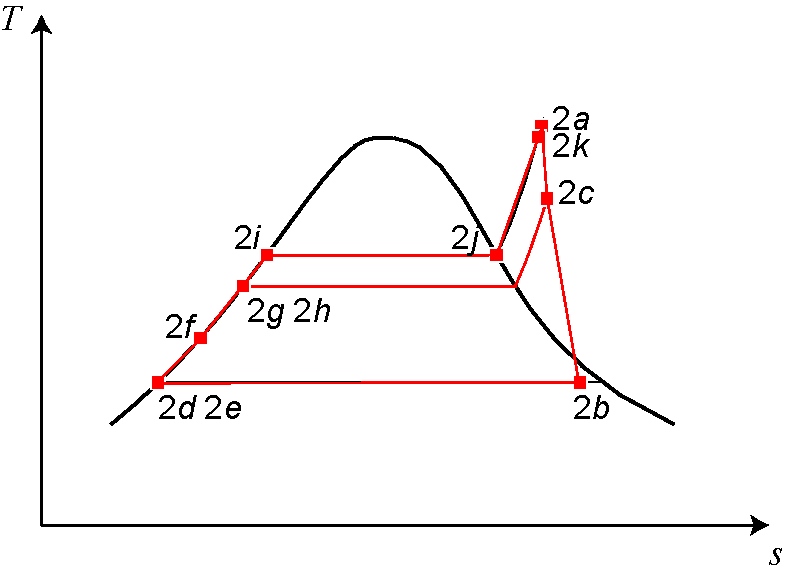
\includegraphics[width = \columnwidth]{fig/Ts_a.pdf}
	\caption{SRC的$T$-$s$图}\label{fig:Ts_Water}
	\end{subfigure}
	~
\begin{subfigure}[b]{0.4\columnwidth}
	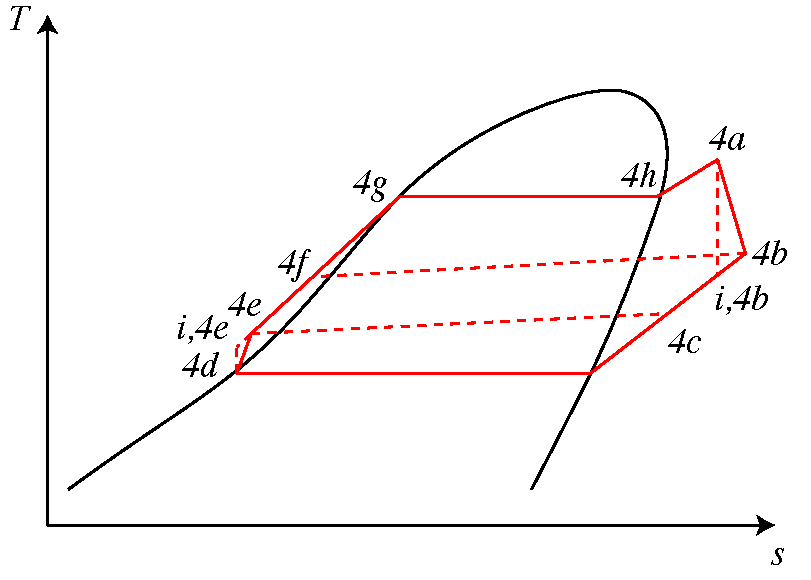
\includegraphics[width = \columnwidth]{fig/Ts_b.pdf}
	\caption{ORC的$T$-$s$图}\label{fig:Ts_organic}
	\end{subfigure}
	\caption{朗肯循环的$T$-$s$图}
	\label{fig:Ts}
\end{figure}
\begin{figure}[htbp]
\centering
	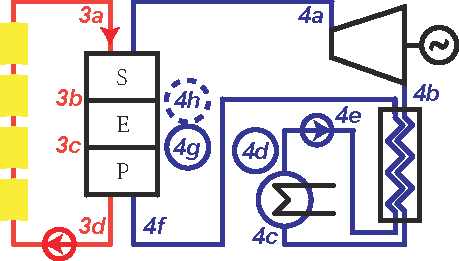
\includegraphics[width = 0.4\columnwidth]{fig/ORCsystem2.pdf}
	\caption{具有回热器的ORC系统结构示意图}
	\label{fig:ORCsystem2}
\end{figure}
汽轮机的相对内效率为
\begin{equation}
  \eta_{i,tb} = (h_{4a}-h_{4b})/(h_{4a}-h_{i,4b})
\end{equation}
其中,$h_{i,4b}$由$s_{4a}$和$p_c$决定。

汽轮机的输出功率为
\begin{equation}
  P_{tb}=\dot{m}_4(h_{4a}-h_{4b})
\end{equation}

过程曲线$4c$-$4d$显示的是凝汽器中的放热曲线。凝汽器的出口流体为饱和液态。出口温度$T_{4d}$和出口焓值$h_{4d}$由汽轮机的出口压力$p_c$决定。

对于回热器,依据能量平衡
\begin{equation}
  h_{4b} - h_{4c} = h_{4f} - h_{4e}
\end{equation}

凝汽器放出的凝结热
\begin{equation}
  Q_{cd} = \dot{m}_4 (h_{4c} - h_{4d})
\end{equation}

泵的功率
\begin{equation}
P_{pu}=\dot{m}_{4}(h_{4e}-h_{4d})
\end{equation}  
其中,$h_{4e}$可以由方程$\eta_{pu} = (h_{i,4e}-h_{4d})/(h_{4e}-h_{4d})$计算得到。$h_{i,4e}$由$s_{4d}$和$p_s$得到。
    
输入朗肯循环的总热量
\begin{equation}
    Q_4=\dot{m}_4(h_{4a}-h_{4f})
\end{equation}

朗肯循环的效率为
\begin{equation}
	\eta_{rk}=\dfrac{P_{tb}-P_{pu}/\eta_{ge}}{\dot{m}_4(h_{4a}-h_{4f})}
\end{equation}

\subsubsection{发电机}
发电机相对而言是独立于梯级系统之外的部件,它的效率一般假定为常数,值为0.975。

\section{蒸汽发生系统建模}
槽式太阳能光热发电厂的蒸汽发生系统可以被分成三部分——预热器、蒸发器和过热器,它们都是换热器。为了便于系统分析,假定这些换热器都不存在流动压力损失,即加热器中的加热流体(以导热油为例)和被加热流体(以水为例)的压力保持不变。水的压力和汽轮机的入口压力相等。此外,假设这些换热器都不与环境交换热量。

为了更加清晰地理解这些换热器的机理建模理论,本文使用\autoref{fig:PES}中的蒸汽发生系统作为例子进行详细分析,其传热过程如\autoref{fig:PES_TQ}所示。

蒸汽发生系统的机理建模过程从本质上来看,是求解各未知状态点的过程。需要再次提出的是,由于水和导热油在换热过程中都没有压降,对于饱和状态,由于其干度已知,其状态是确定的;对于不饱和状态,只要已知温度或焓值,那么其状态也可以确定。这意味着,已知温度可以求出焓值,反之亦然。

\noindent \begin{figure}[ht!]
	\centering
	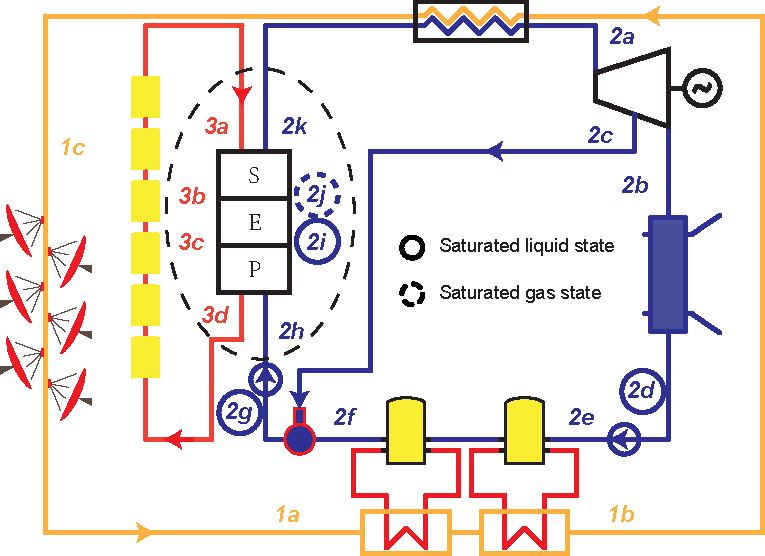
\includegraphics[width = 0.8\columnwidth]{fig/PES}
	\caption{用于分析蒸汽发生系统的梯级系统结构图}
	\label{fig:PES}
\end{figure}

\begin{figure}[ht!]
	\centering
	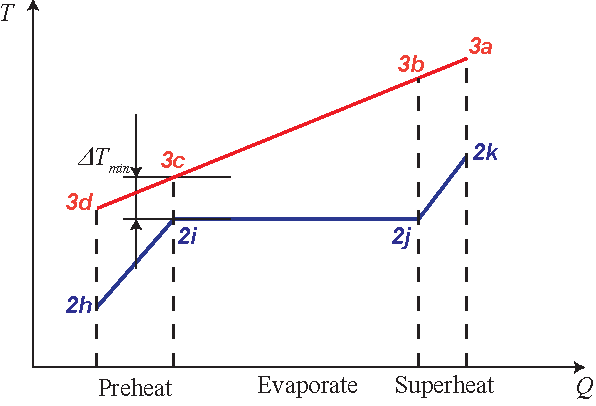
\includegraphics[width = 0.6\columnwidth]{fig/PES_TQ}
	\caption{蒸汽发生过程的$T$-$Q$曲线图}
	\label{fig:PES_TQ}
\end{figure}

对于如\autoref{fig:PES}所示的典型的蒸汽发生系统的建模过程,水工质质量流量$\dot{m}_2$,状态点$2h$和状态点$2k$都由汽轮机及朗肯循环的参数确定,可以看作已知量。状态点$3a$的状态由槽式镜场的设计参数确定,状态点$2i$和$2j$的状态可以由其干度确定。

\begin{enumerate}[label=(\arabic*)]
  \item \emph{预热器}
  
\setlength\parindent{2em}预热器出口的水是饱和液态水($x = 0$),所以其出口温度$T_{2i}$和出口焓值$h_{2i}$由汽轮机的主汽压力$p_s$决定。根据能量平衡方程,
  \begin{equation}
  \dot{m}_3 (h_{3c}-h_{3d})=\dot{m}_2 (h_{2i} - h_{2h})
  \label{eq:preheater}
\end{equation}

  \item \emph{蒸发器}
  
  蒸发器出口的水是饱和蒸汽($x = 1$),所以其出口温度$T_{2j}$和出口焓值$h_{2j}$由汽轮机的主汽压力$p_s$决定。根据能量平衡方程,
  \begin{equation}
  \dot{m}_3 (h_{3b}-h_{3c})=\dot{m}_2 (h_{2j} - h_{2i})
  \label{eq:evaporator}
\end{equation}

	需要指出的是,状态点$3c$的状态由$T_{3c}$决定。而$T_{3c}$由夹点温度(pinch temperature)$\Delta T_{min}$确定,即$T_{3c} = T_{2i} + \Delta T_{min}$。关于夹点温度,\autoref{cha:osgs}有更加详细的说明。
  
  \item \emph{过热器}
  
  根据能量平衡方程,
  \begin{equation}
  \dot{m}_3 (h_{3a}-h_{3b})=\dot{m}_2 (h_{2k} - h_{2j})
  \label{Equation:superheater}
\end{equation}

\end{enumerate}

通过求解\autoref{eq:preheater}到\autoref{Equation:superheater},可以得到导热油的质量流量$\dot{m}_3$和状态点$3b$、$3d$的状态。

\section{梯级系统建模}

由于系统建模采用面向对象的方法,系统是利用各种部件的接口(进出口)相互连接形成的。这些接口通过各股流体(称为流,stream)相互作用。例如\autoref{fig:PES}中的汽轮机和除氧器之间通过抽汽流相互连接。每个流都拥有独立的属性,如流体类型,质量流量,温度,压力,比焓,比熵等等。
为此,利用MATLAB建模工具建立了专门的\textbf{Stream}类,将各流都作为对象进行计算分析。\autoref{cha:MATLAB_SOURCECODE}给出了\textbf{Stream}类的定义的源代码。\textbf{Stream}类中的一些属性由于被多个\textbf{Stream}实例所共用,也被定义为对象。
如\textbf{Stream}类中的属性\textbf{T},\textbf{q\_m}和\textbf{p}也是对象,它们分别属于\textbf{Temperature}类,\textbf{Massflow}类和\textbf{Pressure}类。

给定了\textbf{Stream}对象的固有属性(inherent properties,包括流体类型,质量流量,温度,压力和干度),其依赖属性(dependent properties,包括比焓,比熵和比热容)可以依据其内部方法获得。

如果流是单相流体,它没有干度值,它的依赖属性就可以通过温度和压力获得。如果流是两相流体或饱和流体,那么其干度$0 \leqslant x \leqslant 1$,它的依赖属性可以通过压力和干度获得。选择压力而不是温度作为输入参数的原因是,在梯级系统中,流的压力往往更容易确定。

由于流包含了状态点的所有信息,它被用来记录状态点。梯级系统的模型中创建了多个流对象,用于连接各部件,并记录各部件进出口的状态点信息。各个部件通过流对象连接在一起形成整个系统,流对象也作为参数在各个部件之间传递信息,以完成部件和系统的计算分析及用于结果的展示。
%\subsection{System connection}
不同的部件通过赋值同一个流对象而连接在一起,它们的进出口是连接的接口。
%\subsection{System initialization}
系统通过给定的参数(设计参数)完成初始化,这些参数被赋值给相应的流对象,并影响相关部件的状态。

%\subsection{System calculation}
针对系统计算,需要指出的是,一个部件的某些参数可能和其它多个部件相关联。
在这种条件下,需要使用估值来辅助计算。估值用于设定未定状态的流对象的固有属性(如质量流量或温度),以便于获得流的依赖属性,进而得到状态点的状态信息。这些流对象通过参数传递给相应的部件,进而完成部件内部的计算方法,获得相应的计算结果。这些结果会以状态点参数的形式,和原来设定的估值进行比较。如果估值和相应计算值之间的差异在允许误差范围之内,则接受该估值;否则,估值将会依据隆戈库塔法重新设定,并重新启动部件内的计算,并将新估值和获得的新的计算值进行比较,直至二者之间的差异小于允许误差为止。

例如,在\autoref{fig:PES}所示的蒸汽发生系统中,蒸发器的出口油温%\textbf{evaporator.T\_3o}
还和过热器有关。想要获得该温度值,就需要先使用估值。估值用于赋值给对应于状态点$3b$的流对象的温度属性,这样可以获得该流对象的所有依赖属性(因为其压力已知),包括状态点$3b$的焓值。该流对象作为蒸发器和过热器的输入参数将该状态点相应的焓值带入到蒸发器和过热器中,在蒸发器中通过计算
%方法\textbf{superheater.get\_T\_3i}
得到导热油的质量流量,并在过热器中计算得到过热器的出口油温
%\textbf{superheater.T\_3i}
,并将此值和估值进行比较,如果估值与计算得到的过热器出口油温之差的绝对值
%$\left|\mathrm{evaporator}.T_{3o} - \mathrm{superheater}.T_{3i}\right|$
比允许误差
%($10^{-4}$)
小,则接受该估值;否则,依据隆戈库塔法迭代调整估值,并重新进行计算,直至新估值与计算得到的过热器出口油温之差的绝对值小于允许误差。

\begin{figure}[htbp]
	\centering
	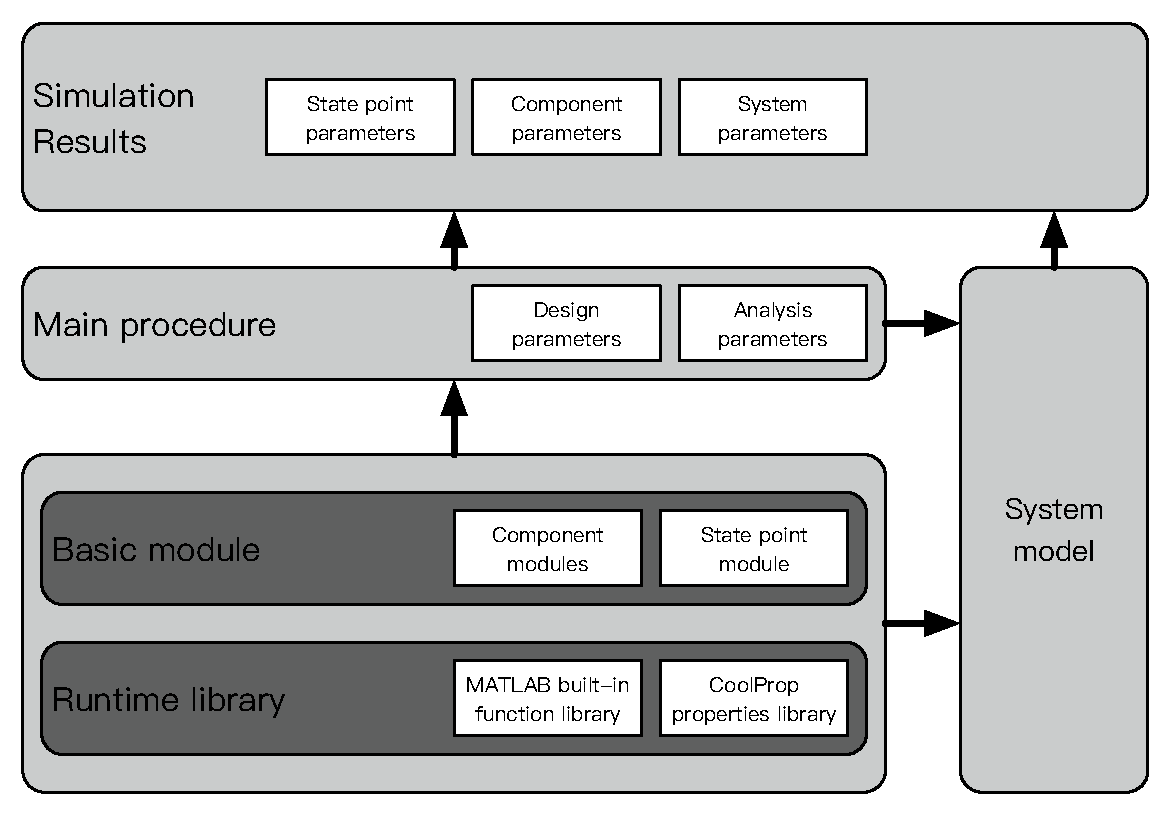
\includegraphics[width = 0.8\columnwidth]{fig/SystemFlow}
	\caption{太阳能光热发电系统设计软件结构图}
	\label{fig:SystemFlow}
\end{figure}

完成各部件的数学机理研究和运行特征分析后,利用MATLAB的数学计算和建模分析等功能,采用面向对象的方式,以运行库文件和各模型基础模块为基础,编写设计软件的主程序,开发了具有软件著作权的太阳能光热发电系统设计软件。\autoref{fig:SystemFlow}是太阳能光热发电系统设计软件结构图。该设计软件具有系统部件选择、部件模型选择、部件连接、设定系统参数、模拟计算、结果分析等功能。
通过该设计软件,可以选择太阳能光热发电系统拓扑结构,连接系统中的各个部件,设定系统初始参数,并进行模拟计算和结果分析,最终实现太阳能光热发电系统的建模,计算和分析工作。

\section{本章小结}

本章分析了太阳能光热梯级系统的建模方法,并详细研究了系统中关键部件和子系统的机理建模。部件模型使用MATLAB建模工具,采用面向对象的方法,部件模型的机理建模充分考虑了各部件的热力学特性,动力学特性以及能量平衡。系统模型采用自底向上的方法,利用部件模型完成系统模型的搭建工作。
基于面向对象语言的封装、组合和多态等特性,各部件间既具有独立性,又具有关联性。所建立的系统模型具有易于搭建,结构清晰,便于替换或改进部件,容易检查单个部件等优点。

系统还专门建立了\textbf{Stream}类用于部件的连接工作,部件的进出口是连接的接口。两个不同的部件通过被赋值同一个流对象而实现相互连接。
此外,本章还简单介绍了不同部件间通过流对象进行耦合计算的方法。

本文还利用MATLAB的数学计算和建模分析等功能,以运行库文件和各模型基础模块为基础,编写设计软件的主程序,完成了具有软件著作权的太阳能光热发电系统设计软件的开发,为本文研究中的大量的建模仿真分析工作提供了坚实的基础。

本文建立的关键部件模型可以通过实验或与经典模型比较等方式进行验证。斯特林机的验证工作表明,与传统的经典的斯特林机模型相比,本文所建立的模型在不同的转速和平均有效压力下,具有与实验数据更接近的性能结果。

\nomenclature[S]{$pu$}{泵} 
\nomenclature[S]{$h$}{加热流体; 齐次解}
\nomenclature[S]{$c$}{冷却流体; 逆流}
\nomenclature{$p_e$}{汽轮机抽汽压力, Pa} 
\nomenclature{$c_p$}{定压比热容, J$\cdot$kg$^{-1}\cdot$K$^{-1}$}
\nomenclature{$T_w$}{壁温, K}
\nomenclature{$A$}{面积, m$^2$}
\nomenclature[S]{$cd$}{凝汽器}
\nomenclature{$Z$}{置换器的往复长度, m}
\nomenclature{$J$}{置换器与圆柱体内壁之间的缝隙大小, m}
\nomenclature[S]{$r$}{回热器}
\nomenclature{$p$}{压力, Pa}
\nomenclature[S]{$cw$}{冷却器壁面}
\nomenclature[S]{$hw$}{加热器壁面}
\nomenclature{$P$}{功率, W}
\nomenclature{$s_{se}$}{斯特林机转速, Hz}
\nomenclature{$x$}{干度}
\nomenclature{$Q$}{吸热量, W}
\nomenclature{$c_v$}{定容比热容, J$\cdot$kg$^{-1}\cdot$K$^{-1}$}
\nomenclature{$k$}{热容比 ($c_p/c_v$);导热率, W$\cdot$m$^{-1}\cdot$K$^{-1}$}
\nomenclature[G]{$\gamma_H$}{过程12的容积率}
\nomenclature[G]{$\gamma_L$}{过程34的容积率}
\nomenclature{$V_E$}{膨胀体积, m$^3$}
\nomenclature{$V_C$}{压缩体积, m$^3$}
\nomenclature{$m_{se}$}{单台斯特林机中的工质的质量, kg}
\nomenclature{$R$}{气体常数, J$\cdot$kg$^{-1}\cdot$K$^{-1}$}
\nomenclature{$V_D$}{死区容积, m$^3$}
\nomenclature{$V_{DH}$}{热头死区容积, m$^3$}
\nomenclature{$V_{DR}$}{回热器死区容积, m$^3$}
\nomenclature{$V_{DC}$}{冷头死区容积, m$^3$}
\nomenclature{$Pr$}{普朗特数}
\nomenclature{$Re$}{雷诺数}
\nomenclature[G]{$\mu$}{动力粘度, kg$\cdot$m$^{-1}$$\cdot$s$^{-1}$}
\nomenclature[S]{$w$}{管壁}
\nomenclature{$Nu$}{努塞尔数}
\nomenclature{$c_r$}{螺旋管的螺旋因子}
\nomenclature[S]{$dr$}{碟式接收器}
\nomenclature[S]{1}{空气} 
\nomenclature[S]{2}{水} 
\nomenclature[S]{3}{导热油}  
\nomenclature[G]{$\delta$}{厚度, m}
\nomenclature[S]{$insu$}{绝热层}
\nomenclature{$l$}{深度, m}
\nomenclature{$d$}{直径, m}
\nomenclature[G]{$\lambda$}{导热率, W$\cdot{}$m$^{-1}$$\cdot$K$^{-1}$}
\nomenclature[G]{$\epsilon$}{发射率}
\nomenclature[G]{$\theta_{dc}$}{碟式集热器开口角度 (0$^{\circ}$表示水平, 90$^{\circ}$表示竖直向下)}
\nomenclature[G]{$\gamma$}{拦截因子;压缩比}
\nomenclature[G]{$\rho$}{反射率}
\nomenclature{$n_g$}{单台斯特林机中的工质的物质的量, mol}
\nomenclature{$U$}{整体换热系数, W$\cdot$m$^{-2}\cdot$K$^{-1}$}
\nomenclature{$q''$}{热流密度, W$\cdot$m$^{-2}$}
\nomenclature{$e$}{回热率}
\nomenclature{$T_R$}{有效回热温度, K}
\nomenclature{$T_L$}{冷腔温度, K}
\nomenclature{$T_H$}{热量温度, K}
\nomenclature{$W$}{输出功, J}
\nomenclature[S]{$th$}{理论值}
\nomenclature{$y$}{汽轮机的抽汽率}
\nomenclature{$K$}{容积因子}